\section{Brodmann Areas}

The functional organization of the cortex into distinct Brodmann areas reflects a deeper principle of regional specialization that extends beyond cytoarchitecture to the molecular level. Each Brodmann area possesses a unique transcriptomic profile - a specific pattern of gene expression that shapes its information processing capabilities and energy management strategies \cite{Amunts2015}. These molecular signatures help explain how different regions maintain distinct functional properties while participating in the broader field of conscious experience.

Unlike the traditional view of Brodmann areas as purely structural divisions, modern neuroscience reveals them as domains of specialized molecular organization \cite{Amunts2007}. Brodmann areas represent distinct regions of the cerebral cortex, first mapped by neuroanatomist Korbinian Brodmann in the early 20th century based on their unique cytoarchitectural organization \cite{Brodmann1909}. These areas differ in the thickness of cortical layers, density of neurons, types of cells present, and patterns of connectivity. Originally identified through careful microscopic examination of cell structure and arrangement, these regions have since been shown to correspond closely with functional specialization in the brain \cite{Eickhoff2018}.

Each Brodmann area exhibits characteristic properties that reflect its role in processing specific types of information. For example, primary visual cortex (Brodmann area 17) shows a prominent layer 4 that receives direct thalamic input, while motor cortex (Brodmann area 4) is characterized by large pyramidal neurons in layer 5 that project to the spinal cord \cite{Zilles2010}. These structural differences support each region's specialized function while maintaining the capacity to integrate into broader conscious processes.

The functional organization of the cortex into distinct regions, mapped through careful cytoarchitectural analysis, takes on profound new significance when examined through the framework of energetically coherent computation. Far from being merely anatomical subdivisions, these areas represent domains of specialized molecular organization that enable distinct patterns of energetic coherence while maintaining integration with broader conscious processes \cite{Glasser2016}.

Unlike the traditional view of Brodmann areas as purely structural divisions, modern neuroscience reveals them as domains of sophisticated molecular organization \cite{Hawrylycz2012}. Each area maintains unique transcriptomic profiles that shape its capacity for information processing and energy management. These molecular signatures help explain how different regions maintain distinct functional properties while participating in the broader field of conscious experience.

The cellular architecture of each Brodmann area reflects evolutionary optimization for specific forms of information processing \cite{Palomero-Gallagher2019}. Areas devoted to sensory processing, such as primary visual cortex, demonstrate precisely organized cellular arrangements that support rapid, parallel processing of sensory inputs. In contrast, association areas maintain more flexible architectures that enable complex integration of information from multiple sources. These structural differences support each region's specialized function while maintaining the capacity for integration into broader conscious processes.

\begin{figure}[h]
    \centering
    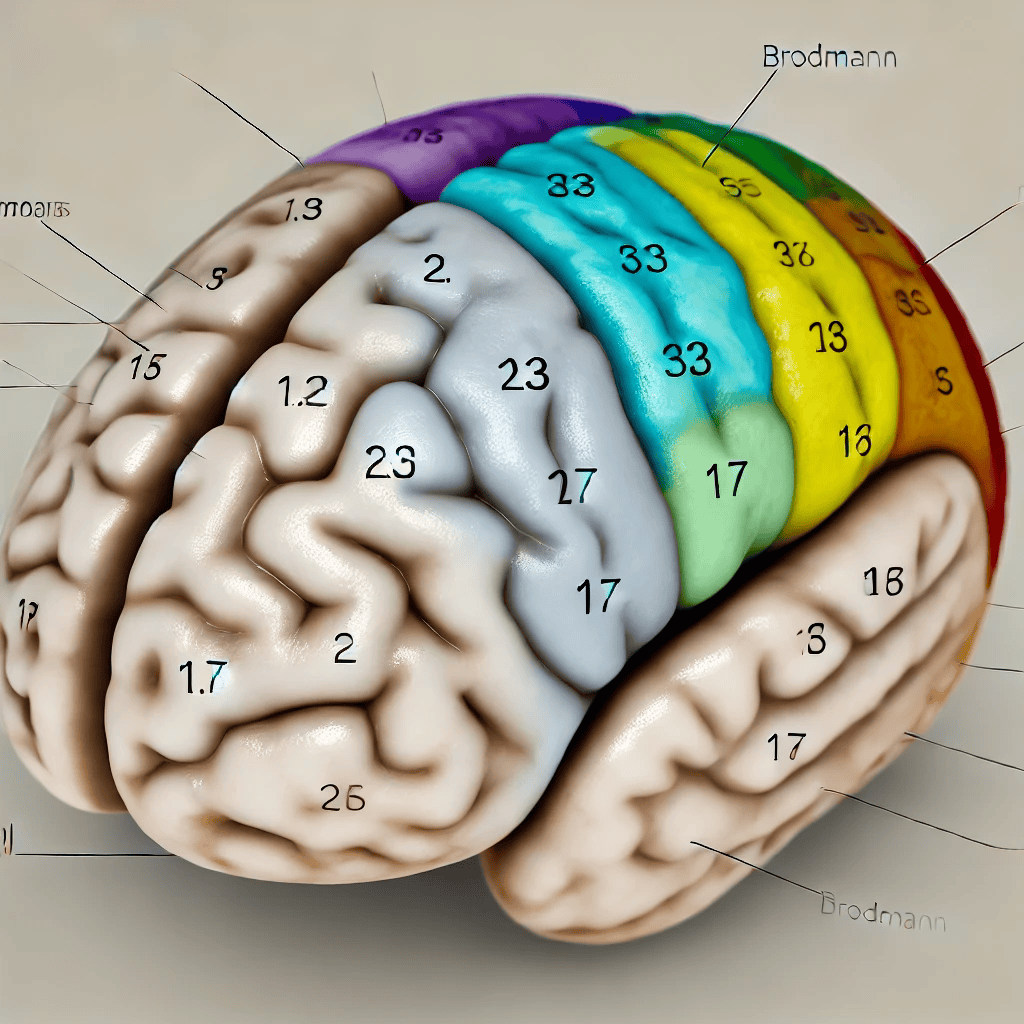
\includegraphics[width=0.8\textwidth]{brodmann.png}

    \caption{Brodmann areas align with great variation in transcriptomic profiles}
\end{figure}

The relationship between cellular organization and energetic coherence becomes particularly evident when examining how different Brodmann areas process information \cite{Passingham2002}. Primary sensory areas maintain tightly organized columns that enable precise mapping of sensory inputs while supporting stable patterns of energetic coherence. Association areas demonstrate more distributed patterns of organization that allow for flexible integration of information while maintaining coherent energy states across larger spatial domains.

Transcriptomic analysis reveals how each Brodmann area expresses distinct combinations of ion channels, receptors, and metabolic enzymes that shape its functional properties \cite{Lake2018}. These molecular profiles determine not just the computational capabilities of each region but also its capacity for maintaining specific patterns of energetic coherence. The resulting specialization enables sophisticated processing of different types of information while supporting integration into unified conscious experiences.

The patterns of connectivity between Brodmann areas reflect both computational requirements and energetic constraints \cite{VanEssen2012}. Long-range connections between regions must balance the need for efficient information transfer against the metabolic costs of maintaining extended axonal processes. This optimization creates networks that can support complex conscious processing while respecting fundamental energetic limitations.

The hierarchical organization of Brodmann areas reveals sophisticated principles of information processing and energy management \cite{Amunts2015}. Primary sensory areas maintain relatively rigid patterns of coherence that enable faithful representation of sensory inputs, while higher association areas demonstrate more flexible organizations that support abstract thought and complex integration. This hierarchy reflects not just computational specialization but different strategies for maintaining energetic coherence across varying temporal and spatial scales.

Understanding how Brodmann areas maintain distinct functional properties while enabling unified conscious experience represents a crucial challenge for consciousness research \cite{Scholtens2014}. The solution appears to lie in how each area achieves its specialized processing through unique patterns of energetic coherence that remain compatible with broader integration. This balance between specialization and integration emerges from the precise molecular and cellular organization of each region.

Building on the pioneering work of early neuroanatomists \cite{Vogt1919}, modern research has revealed increasingly sophisticated understanding of how regional specialization supports conscious processing. The precise laminar organization and cell-type distributions within each Brodmann area create the conditions necessary for maintaining specific patterns of energetic coherence while enabling integration into broader conscious states.

Perhaps most significantly, the study of Brodmann areas through ECC's framework suggests new approaches to understanding both normal conscious processing and pathological conditions \cite{Amunts2015}. Disorders affecting specific Brodmann areas may disrupt consciousness not just through loss of particular functions but through perturbation of broader patterns of energetic coherence. This perspective suggests novel therapeutic approaches targeting the restoration of normal energy dynamics rather than focusing solely on specific cellular pathologies.

The implications extend beyond clinical applications to fundamental questions about the nature of conscious experience \cite{Palomero-Gallagher2019}. The precise organization of Brodmann areas demonstrates how biological systems can achieve both specialized processing and global integration through sophisticated management of energetic coherence. This understanding proves essential for any complete theory of consciousness and suggests new directions for developing artificial systems capable of supporting conscious-like processing.

Recent advances in mapping brain organization have revealed increasingly complex patterns of regional specialization that extend beyond classical Brodmann parcellation \cite{Hawrylycz2012}. These findings suggest that the fundamental principles of regional organization - the careful balance between specialization and integration, the maintenance of specific energy dynamics, and the creation of stable processing domains - operate across multiple spatial scales.

The study of Brodmann areas thus reveals fundamental principles about how conscious processing emerges from neural organization \cite{Eickhoff2018}. Rather than representing arbitrary subdivisions, these regions reflect deep organizational principles that enable sophisticated information processing while maintaining the specific patterns of energetic coherence necessary for conscious experience. Understanding these principles proves crucial for both theoretical advances in consciousness studies and practical applications in treating neurological disorders.

Building on our understanding of regional specialization in the cortex, we must now examine how specific patterns of gene expression shape the capacity for conscious processing across different brain regions. These transcriptomic profiles create what ECC terms the "rich alphabet" of possible neural states, enabling sophisticated information processing while maintaining energetic coherence \cite{Lake2018}.